\documentclass{standalone}
\usepackage{tikz}
\usetikzlibrary{patterns, positioning}
\usepackage[sfdefault]{ClearSans} %% option 'sfdefault' activates Clear Sans as the default text font
\usepackage[T1]{fontenc}

\begin{document}
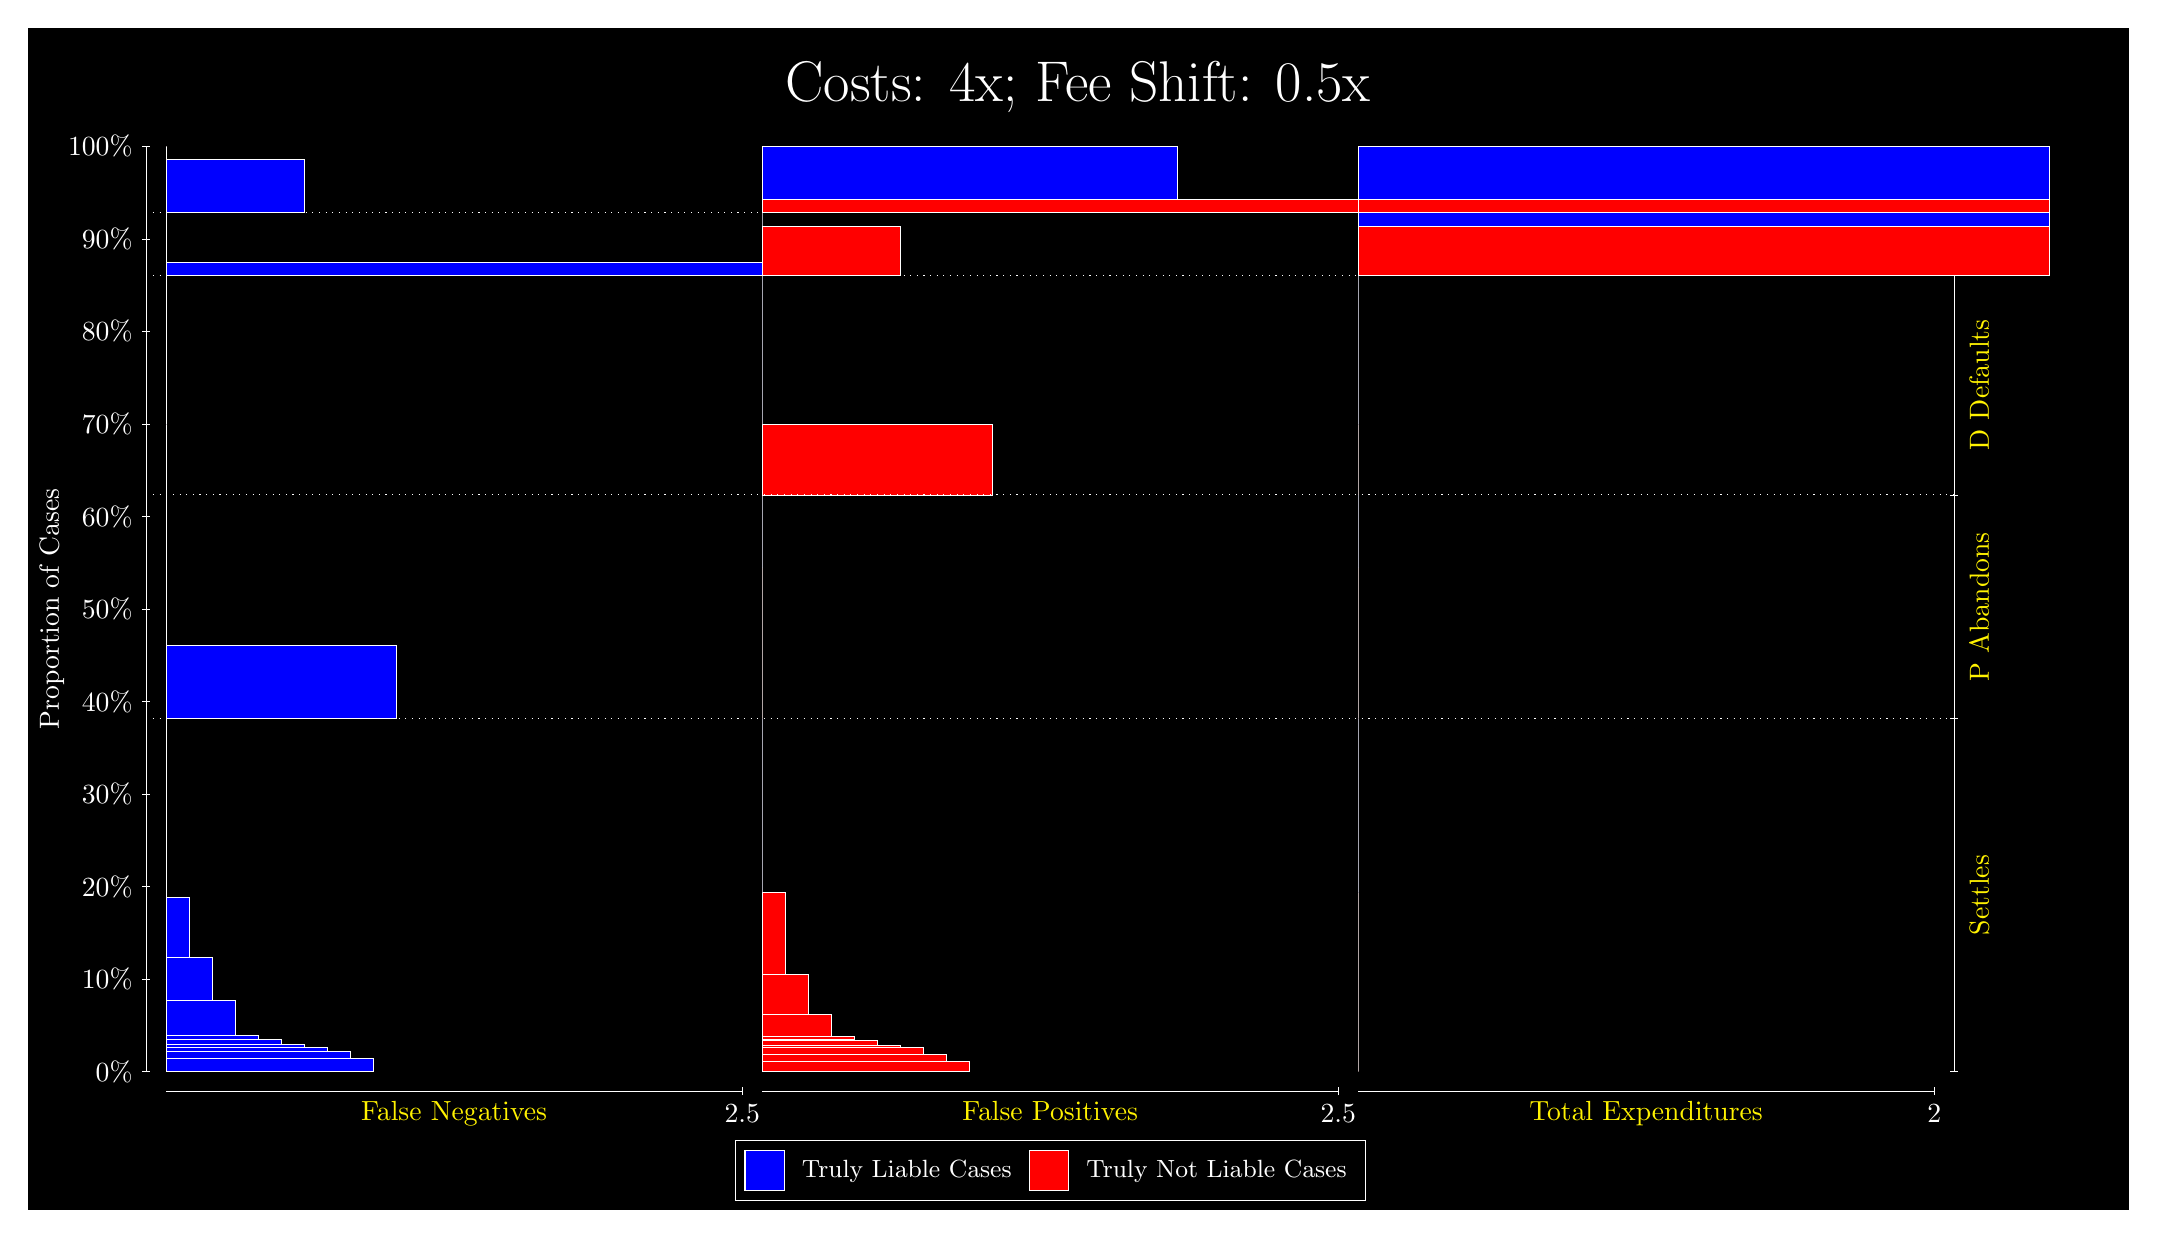
\begin{tikzpicture}
\draw[fill=black] (0,0) rectangle (26.667,15);
\draw[text=white] (0,13.5) rectangle (26.667,15) node[midway] {\huge Costs: 4x; Fee Shift: 0.5x};
\draw[white, very thin] (1.5,1.75) -- (1.5,13.5);
\node[rotate=90, text=white, anchor=center] at (0.3, 7.625) {Proportion of Cases};
\draw[white, very thin] (1.45,1.75) -- (1.55,1.75);
\node[text=white, anchor=east] at (1.45, 1.75) {0\%};
\draw[white, very thin] (1.45,2.925) -- (1.55,2.925);
\node[text=white, anchor=east] at (1.45, 2.925) {10\%};
\draw[white, very thin] (1.45,4.1) -- (1.55,4.1);
\node[text=white, anchor=east] at (1.45, 4.1) {20\%};
\draw[white, very thin] (1.45,5.275) -- (1.55,5.275);
\node[text=white, anchor=east] at (1.45, 5.275) {30\%};
\draw[white, very thin] (1.45,6.45) -- (1.55,6.45);
\node[text=white, anchor=east] at (1.45, 6.45) {40\%};
\draw[white, very thin] (1.45,7.625) -- (1.55,7.625);
\node[text=white, anchor=east] at (1.45, 7.625) {50\%};
\draw[white, very thin] (1.45,8.8) -- (1.55,8.8);
\node[text=white, anchor=east] at (1.45, 8.8) {60\%};
\draw[white, very thin] (1.45,9.975) -- (1.55,9.975);
\node[text=white, anchor=east] at (1.45, 9.975) {70\%};
\draw[white, very thin] (1.45,11.15) -- (1.55,11.15);
\node[text=white, anchor=east] at (1.45, 11.15) {80\%};
\draw[white, very thin] (1.45,12.325) -- (1.55,12.325);
\node[text=white, anchor=east] at (1.45, 12.325) {90\%};
\draw[white, very thin] (1.45,13.5) -- (1.55,13.5);
\node[text=white, anchor=east] at (1.45, 13.5) {100\%};

\draw[white, very thin] (24.457,1.75) -- (24.457,13.5);
\draw[white, very thin] (24.407,1.75) -- (24.507,1.75);
\node[anchor=west] at (24.407, 1.75) {};
\draw[white, very thin] (24.407,6.2327) -- (24.507,6.2327);
\node[anchor=west] at (24.407, 6.2327) {};
\draw[white, very thin] (24.407,9.0731) -- (24.507,9.0731);
\node[anchor=west] at (24.407, 9.0731) {};
\draw[white, very thin] (24.407,11.864) -- (24.507,11.864);
\node[anchor=west] at (24.407, 11.864) {};
\draw[white, very thin] (24.407,12.658) -- (24.507,12.658);
\node[anchor=west] at (24.407, 12.658) {};
\draw[white, very thin] (24.407,13.5) -- (24.507,13.5);
\node[anchor=west] at (24.407, 13.5) {};

\draw[white, very thin, fill=blue] (1.75,1.75) rectangle (4.3848,1.9213);
\draw[white, very thin, fill=blue] (1.75,1.9213) rectangle (4.092,2.0022);
\draw[white, very thin, fill=blue] (1.75,2.0022) rectangle (3.7993,2.0602);
\draw[white, very thin, fill=blue] (1.75,2.0602) rectangle (3.5065,2.0903);
\draw[white, very thin, fill=blue] (1.75,2.0903) rectangle (3.5065,2.0944);
\draw[white, very thin, fill=blue] (1.75,2.0944) rectangle (3.2138,2.1594);
\draw[white, very thin, fill=blue] (1.75,2.1594) rectangle (2.921,2.2122);
\draw[white, very thin, fill=blue] (1.75,2.2122) rectangle (2.6283,2.652);
\draw[white, very thin, fill=blue] (1.75,2.652) rectangle (2.3355,3.204);
\draw[white, very thin, fill=blue] (1.75,3.204) rectangle (2.0428,3.9619);
\draw[white, very thin, fill=red] (1.75,3.9619) rectangle (1.75,6.2327);
\draw[white, very thin, fill=blue] (1.75,6.2327) rectangle (4.6775,7.1585);
\draw[white, very thin, fill=red] (1.75,7.1585) rectangle (1.75,9.0731);
\draw[white, very thin, fill=red] (1.75,9.0731) rectangle (1.75,9.9688);
\draw[white, very thin, fill=blue] (1.75,9.9688) rectangle (1.75,11.864);
\draw[white, very thin, fill=blue] (1.75,11.864) rectangle (9.9471,12.033);
\draw[white, very thin, fill=red] (1.75,12.033) rectangle (1.75,12.658);
\draw[white, very thin, fill=blue] (1.75,12.658) rectangle (3.5065,13.331);
\draw[white, very thin, fill=red] (1.75,13.331) rectangle (1.75,13.5);
\draw[white, very thin, fill=red] (9.3189,1.75) rectangle (11.954,1.8799);
\draw[white, very thin, fill=red] (9.3189,1.8799) rectangle (11.661,1.9719);
\draw[white, very thin, fill=red] (9.3189,1.9719) rectangle (11.368,2.0559);
\draw[white, very thin, fill=red] (9.3189,2.0559) rectangle (11.075,2.0838);
\draw[white, very thin, fill=red] (9.3189,2.0838) rectangle (10.783,2.1482);
\draw[white, very thin, fill=red] (9.3189,2.1482) rectangle (10.49,2.1618);
\draw[white, very thin, fill=red] (9.3189,2.1618) rectangle (10.49,2.2009);
\draw[white, very thin, fill=red] (9.3189,2.2009) rectangle (10.197,2.4775);
\draw[white, very thin, fill=red] (9.3189,2.4775) rectangle (9.9044,2.9811);
\draw[white, very thin, fill=red] (9.3189,2.9811) rectangle (9.6116,4.0208);
\draw[white, very thin, fill=blue] (9.3189,4.0208) rectangle (9.3189,6.2327);
\draw[white, very thin, fill=red] (9.3189,6.2327) rectangle (9.3189,8.1473);
\draw[white, very thin, fill=blue] (9.3189,8.1473) rectangle (9.3189,9.0731);
\draw[white, very thin, fill=red] (9.3189,9.0731) rectangle (12.246,9.9688);
\draw[white, very thin, fill=blue] (9.3189,9.9688) rectangle (9.3189,11.864);
\draw[white, very thin, fill=red] (9.3189,11.864) rectangle (11.075,12.49);
\draw[white, very thin, fill=blue] (9.3189,12.49) rectangle (9.3189,12.658);
\draw[white, very thin, fill=red] (9.3189,12.658) rectangle (17.516,12.827);
\draw[white, very thin, fill=blue] (9.3189,12.827) rectangle (14.588,13.5);
\draw[white, very thin, fill=red] (16.888,1.75) rectangle (16.888,4.0208);
\draw[white, very thin, fill=blue] (16.888,4.0208) rectangle (16.888,6.2327);
\draw[white, very thin, fill=red] (16.888,6.2327) rectangle (16.888,8.1473);
\draw[white, very thin, fill=blue] (16.888,8.1473) rectangle (16.888,9.0731);
\draw[white, very thin, fill=red] (16.888,9.0731) rectangle (16.888,9.9688);
\draw[white, very thin, fill=blue] (16.888,9.9688) rectangle (16.888,11.864);
\draw[white, very thin, fill=red] (16.888,11.864) rectangle (25.67,12.49);
\draw[white, very thin, fill=blue] (16.888,12.49) rectangle (25.67,12.658);
\draw[white, very thin, fill=red] (16.888,12.658) rectangle (25.67,12.827);
\draw[white, very thin, fill=blue] (16.888,12.827) rectangle (25.67,13.5);
\draw[white, dotted] (1.5,6.2327) -- (24.457,6.2327);
\draw[white, dotted] (1.5,9.0731) -- (24.457,9.0731);
\draw[white, dotted] (1.5,11.864) -- (24.457,11.864);
\draw[white, dotted] (1.5,12.658) -- (24.457,12.658);
\draw[white, very thin] (1.75,1.5) -- (9.0689,1.5);
\node[text=yellow, anchor=north] at (5.4094, 1.5) {False Negatives};
\draw[white, very thin] (9.0689,1.45) -- (9.0689,1.55);
\node[text=white, anchor=north] at (9.0689, 1.45) {2.5};

\draw[white, very thin] (9.3189,1.5) -- (16.638,1.5);
\node[text=yellow, anchor=north] at (12.978, 1.5) {False Positives};
\draw[white, very thin] (16.638,1.45) -- (16.638,1.55);
\node[text=white, anchor=north] at (16.638, 1.45) {2.5};

\draw[white, very thin] (16.888,1.5) -- (24.207,1.5);
\node[text=yellow, anchor=north] at (20.547, 1.5) {Total Expenditures};
\draw[white, very thin] (24.207,1.45) -- (24.207,1.55);
\node[text=white, anchor=north] at (24.207, 1.45) {2};

\node[text=yellow, centered, rotate=90] at (24.777, 3.9914) {Settles};
\node[text=yellow, centered, rotate=90] at (24.777, 7.6529) {P Abandons};
\node[text=yellow, centered, rotate=90] at (24.777, 10.469) {D Defaults};



\draw (12.978300999999998,1.5) node[draw=none] (baseCoordinate) {};
\begin{scope}[align=center]
        \matrix[scale=0.5, draw=white, below=0.5cm of baseCoordinate, nodes={draw}, column sep=0.1cm]{
            \node[rectangle, draw, minimum width=0.5cm, minimum height=0.5cm, fill=blue] {}; &
            \node[draw=none, font=\small, text=white] (B) {Truly Liable Cases}; &
            \node[rectangle, draw, minimum width=0.5cm, minimum height=0.5cm, fill=red] {}; &
            \node[draw=none, font=\small, text=white] (B) {Truly Not Liable Cases}; \\
            };
\end{scope}

\end{tikzpicture}
\end{document}